\section{Example Usage of the hws Library}
\label{sec:hws_example}

\begin{listing}
    \begin{moderncode}[highlightlines={2, 5-6, 18-19}]{python}
import plssvm
import HardwareSampling as hws
from sklearn.datasets import make_classification as mc

sampler = hws.SystemHardwareSampler()
sampler.start()

sampler.add_event("create")
X, y = mc(n_samples=2**17, n_features=2**11)
svc = plssvm.svm.SVC(C=1.0, tol=1e-8)

sampler.add_event("fit")
svc.fit(X, y)

sampler.add_event("score")
print(f"model accuracy: {svc.score(X, y)}")

sampler.stop()
sampler.dump_yaml("samples.yaml")
    \end{moderncode}
    \caption{%
    A code example showing the simplicity of the hws library. 
    With only five required lines of code, it is possible to gather information from the whole system. 
    Additionally, events can be added to make the final output easier to understand and post-process (lines 8, 12, and 15).
    }
    \label{code:hws_python}
\end{listing}

After the theoretical descriptions of the hws library in the last sections, this section gives a practical example using hws' Python bindings shown in \autoref{code:hws_python}. 
The only required lines to collect hardware samples with hws are highlighted. 
In line 5, the used hardware sampler is created. 
The example uses a \code{SystemHardwareSampler}, automatically gathering information from all available and supported hardware platforms in the current system. 
Alternatively, one or more hardware-specific hardware samplers could have been used. 
Since no constructor parameters are provided, all categories are sampled, and the default sampling interval is used. 
In the next line, sampling is started. 
After this, everything is sampled until line 18, where sampling is stopped. 
In line 19, the gathered information is saved to a YAML file. 
Additionally, events can be added to make the final output easier to understand and post-process. 
Although only the Python bindings are shown, the code would look nearly identical when using \cpp since the Python bindings are closely modeled after the \cpp functions and classes. 

\begin{listing}
    \begin{moderncode}{yaml}
# the sample category
clock:
  # an exemplary turbostat entry;
  # contains the original turbostat column header name
  average_non_idle_clock_frequency:
    turbostat_name: "Bzy_MHz"
    unit: "MHz"
    values: [3932, 4261, 3525, 3924]
    
  # an exemplary NVML NVIDIA GPU entry
  clock_frequency_max:
    unit: "MHz"
    values: 1440
    \end{moderncode}
    \caption{%
    Exemplary YAML entries. 
    Note that the comments are not output in the YAML file but are only added to this example to facilitate explanation. 
    }
    \label{code:hws_yaml}
\end{listing}

An excerpt from an example YAML file created after the call to the \code{dump_yaml} function is shown in \autoref{code:hws_yaml}. 
The samples are grouped into the different sample categories previously introduced. 
All YAML entries have roughly the same structure: a unit and a value. 
The unit can either be a physical unit like $\si{\mega\hertz}$ in the example, but also, e.g, a simple \texttt{string} in case of the hardware name. 
The second entry is either a single value for fixed samples or a YAML array containing all sampled values. 
In the case of \gls{cpu} entries created via turbostat, the original turbostat header name is also included. 
In addition to the samples, the hardware platform's name, a timestamp when the sampling started, the potential events, the sampling interval, and the time points when the samples were gathered are always reported in the YAML file. 

\begin{figure}
    \centering
    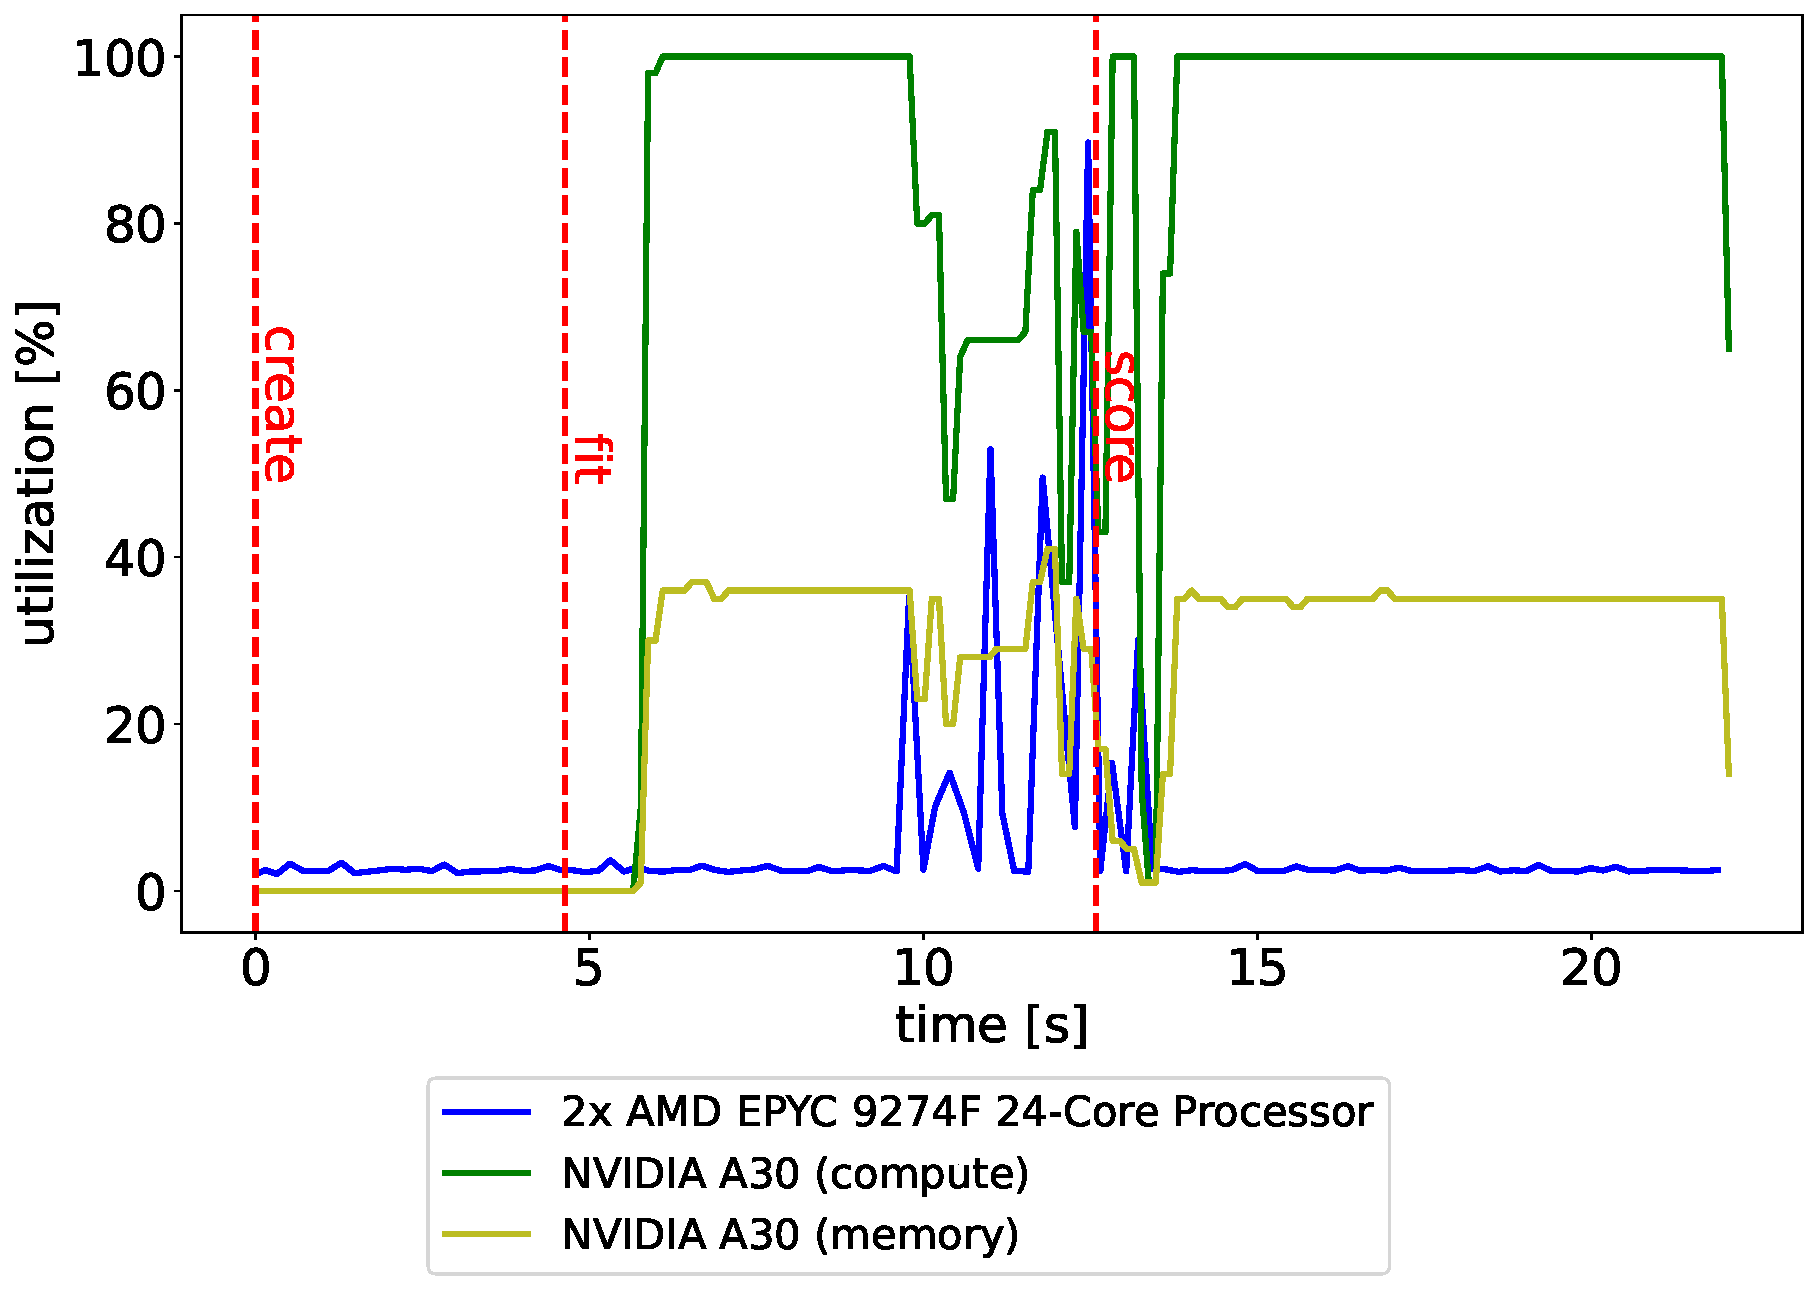
\includegraphics[width=0.85\linewidth]{figures/03_performance_sampling_hws/utilization.pdf}
    \caption{%
    The compute and memory utilization of the code shown in \autoref{code:hws_python} executed on a machine with dual-socket \gls{amd} EPYC 9274F \glspl{cpu} and an NVIDIA A30 \gls{gpu}. 
    }
    \label{fig:hws_plot_example}
\end{figure}

This YAML file can be parsed, e.g., using the PyYAML Python library~\cite{simonov_pyyaml_2024} and used to create a plot similar to the one shown in \autoref{fig:hws_plot_example}.
The code from \autoref{code:hws_python} was run on a system with dual-socket \gls{amd} EPYC 9274F \glspl{cpu} and an NVIDIA A30 \gls{gpu}. 

\todo{PLOT + beschreiben}